\documentclass[11pt, a4paper]{article}
\usepackage{pdfpages}
\usepackage{parallel}
\usepackage[T2A]{fontenc}
\usepackage{ucs}
\usepackage[utf8x]{inputenc}
\usepackage[polish,english,russian]{babel}
\usepackage{hyperref}
\usepackage{rotating}
\usepackage[inner=2cm,top=1.8cm,outer=2cm,bottom=2.3cm,nohead]{geometry}
\usepackage{listings}
\usepackage{graphicx}
\usepackage{wrapfig}
\usepackage{longtable}
\usepackage{indentfirst}
\usepackage{array}
\usepackage{tikzsymbols}
\usepackage{soul}
\usepackage[ruled,vlined]{algorithm2e}
%\counterwithout{figure}{section} 

\usepackage{url}
\makeatletter
\g@addto@macro{\UrlBreaks}{\UrlOrds}
\makeatother

\newcolumntype{P}[1]{>{\raggedright\arraybackslash}p{#1}}
\frenchspacing
\usepackage{fixltx2e} %text sub- and superscripts
\usepackage{icomma} % коскі ў матэматычным рэжыме
\PreloadUnicodePage{4}

\newcommand{\longpage}{\enlargethispage{\baselineskip}}
\newcommand{\shortpage}{\enlargethispage{-\baselineskip}}

\def\switchlang#1{\expandafter\csname switchlang#1\endcsname}
\def\switchlangbe{
\let\saverefname=\refname%
\def\refname{Літаратура}%
\def\figurename{Іл.}%
}
\def\switchlangen{
\let\saverefname=\refname%
\def\refname{References}%
\def\figurename{Fig.}%
}
\def\switchlangru{
\let\saverefname=\refname%
\let\savefigurename=\figurename%
\def\refname{Литература}%
\def\figurename{Рис.}%
}

\hyphenation{admi-ni-stra-tive}
\hyphenation{ex-pe-ri-ence}
\hyphenation{fle-xi-bi-li-ty}
\hyphenation{Py-thon}
\hyphenation{ma-the-ma-ti-cal}
\hyphenation{re-ported}
\hyphenation{imp-le-menta-tions}
\hyphenation{pro-vides}
\hyphenation{en-gi-neering}
\hyphenation{com-pa-ti-bi-li-ty}
\hyphenation{im-pos-sible}
\hyphenation{desk-top}
\hyphenation{elec-tro-nic}
\hyphenation{com-pa-ny}
\hyphenation{de-ve-lop-ment}
\hyphenation{de-ve-loping}
\hyphenation{de-ve-lop}
\hyphenation{da-ta-ba-se}
\hyphenation{plat-forms}
\hyphenation{or-ga-ni-za-tion}
\hyphenation{pro-gramming}
\hyphenation{in-stru-ments}
\hyphenation{Li-nux}
\hyphenation{sour-ce}
\hyphenation{en-vi-ron-ment}
\hyphenation{Te-le-pathy}
\hyphenation{Li-nux-ov-ka}
\hyphenation{Open-BSD}
\hyphenation{Free-BSD}
\hyphenation{men-ti-on-ed}
\hyphenation{app-li-ca-tion}

\def\progref!#1!{\texttt{#1}}
\renewcommand{\arraystretch}{2} %Іначай формулы ў матрыцы зліпаюцца з лініямі
\usepackage{array}

\def\interview #1 (#2), #3, #4, #5\par{

\section[#1, #3, #4]{#1 -- #3, #4}
\def\qname{LVEE}
\def\aname{#1}
\def\q ##1\par{{\noindent \bf \qname: ##1 }\par}
\def\a{{\noindent \bf \aname: } \def\qname{L}\def\aname{#2}}
}

\def\interview* #1 (#2), #3, #4, #5\par{

\section*{#1\\{\small\rm #3, #4. #5}}
\ifx\ParallelWhichBox\undefined%
    \addcontentsline{toc}{section}{#1, #3, #4}%
\else%
\ifnum\ParallelWhichBox=0%
    \addcontentsline{toc}{section}{#1, #3, #4}%
\fi\fi%

\def\qname{LVEE}
\def\aname{#1}
\def\q ##1\par{{\noindent \bf \qname: ##1 }\par}
\def\a{{\noindent \bf \aname: } \def\qname{L}\def\aname{#2}}
}

\newcommand{\interviewfooter}[1]{
\vskip 1em
\noindent \textit{#1}
}

\switchlang{en}
\begin{document}

\title{2000 -- Celltrix/Loas Ball Less Mouse}
\date{}
\maketitle
\selectlanguage{english}

The Ball Less Mouse, also designated by model number MUS-P241SL (fig. \ref{fig:BallLessMousePic}) was introduced to the Japanese market in 2000 by Loas, a company specializing in the manufacture and sales of computer furniture, supplies, and other computer-related products \cite{loas}. As an integrator, Loas actively marketed products from other manufacturers under its own brand. Specifically, the development and production of the MUS-P241SL were carried out by the Taiwanese company Celltrix Technology, best known for the Celtrix Trackbar (an alternative cursor control device based on a rolling cylinder). The design of the Ball Less Mouse is equally unusual: it appears to be the last computer mouse based on the 1973 Xerox patent describing motion tracking based on two orthogonal wheels \cite{pat}.

\begin{figure}[h]
    \centering
    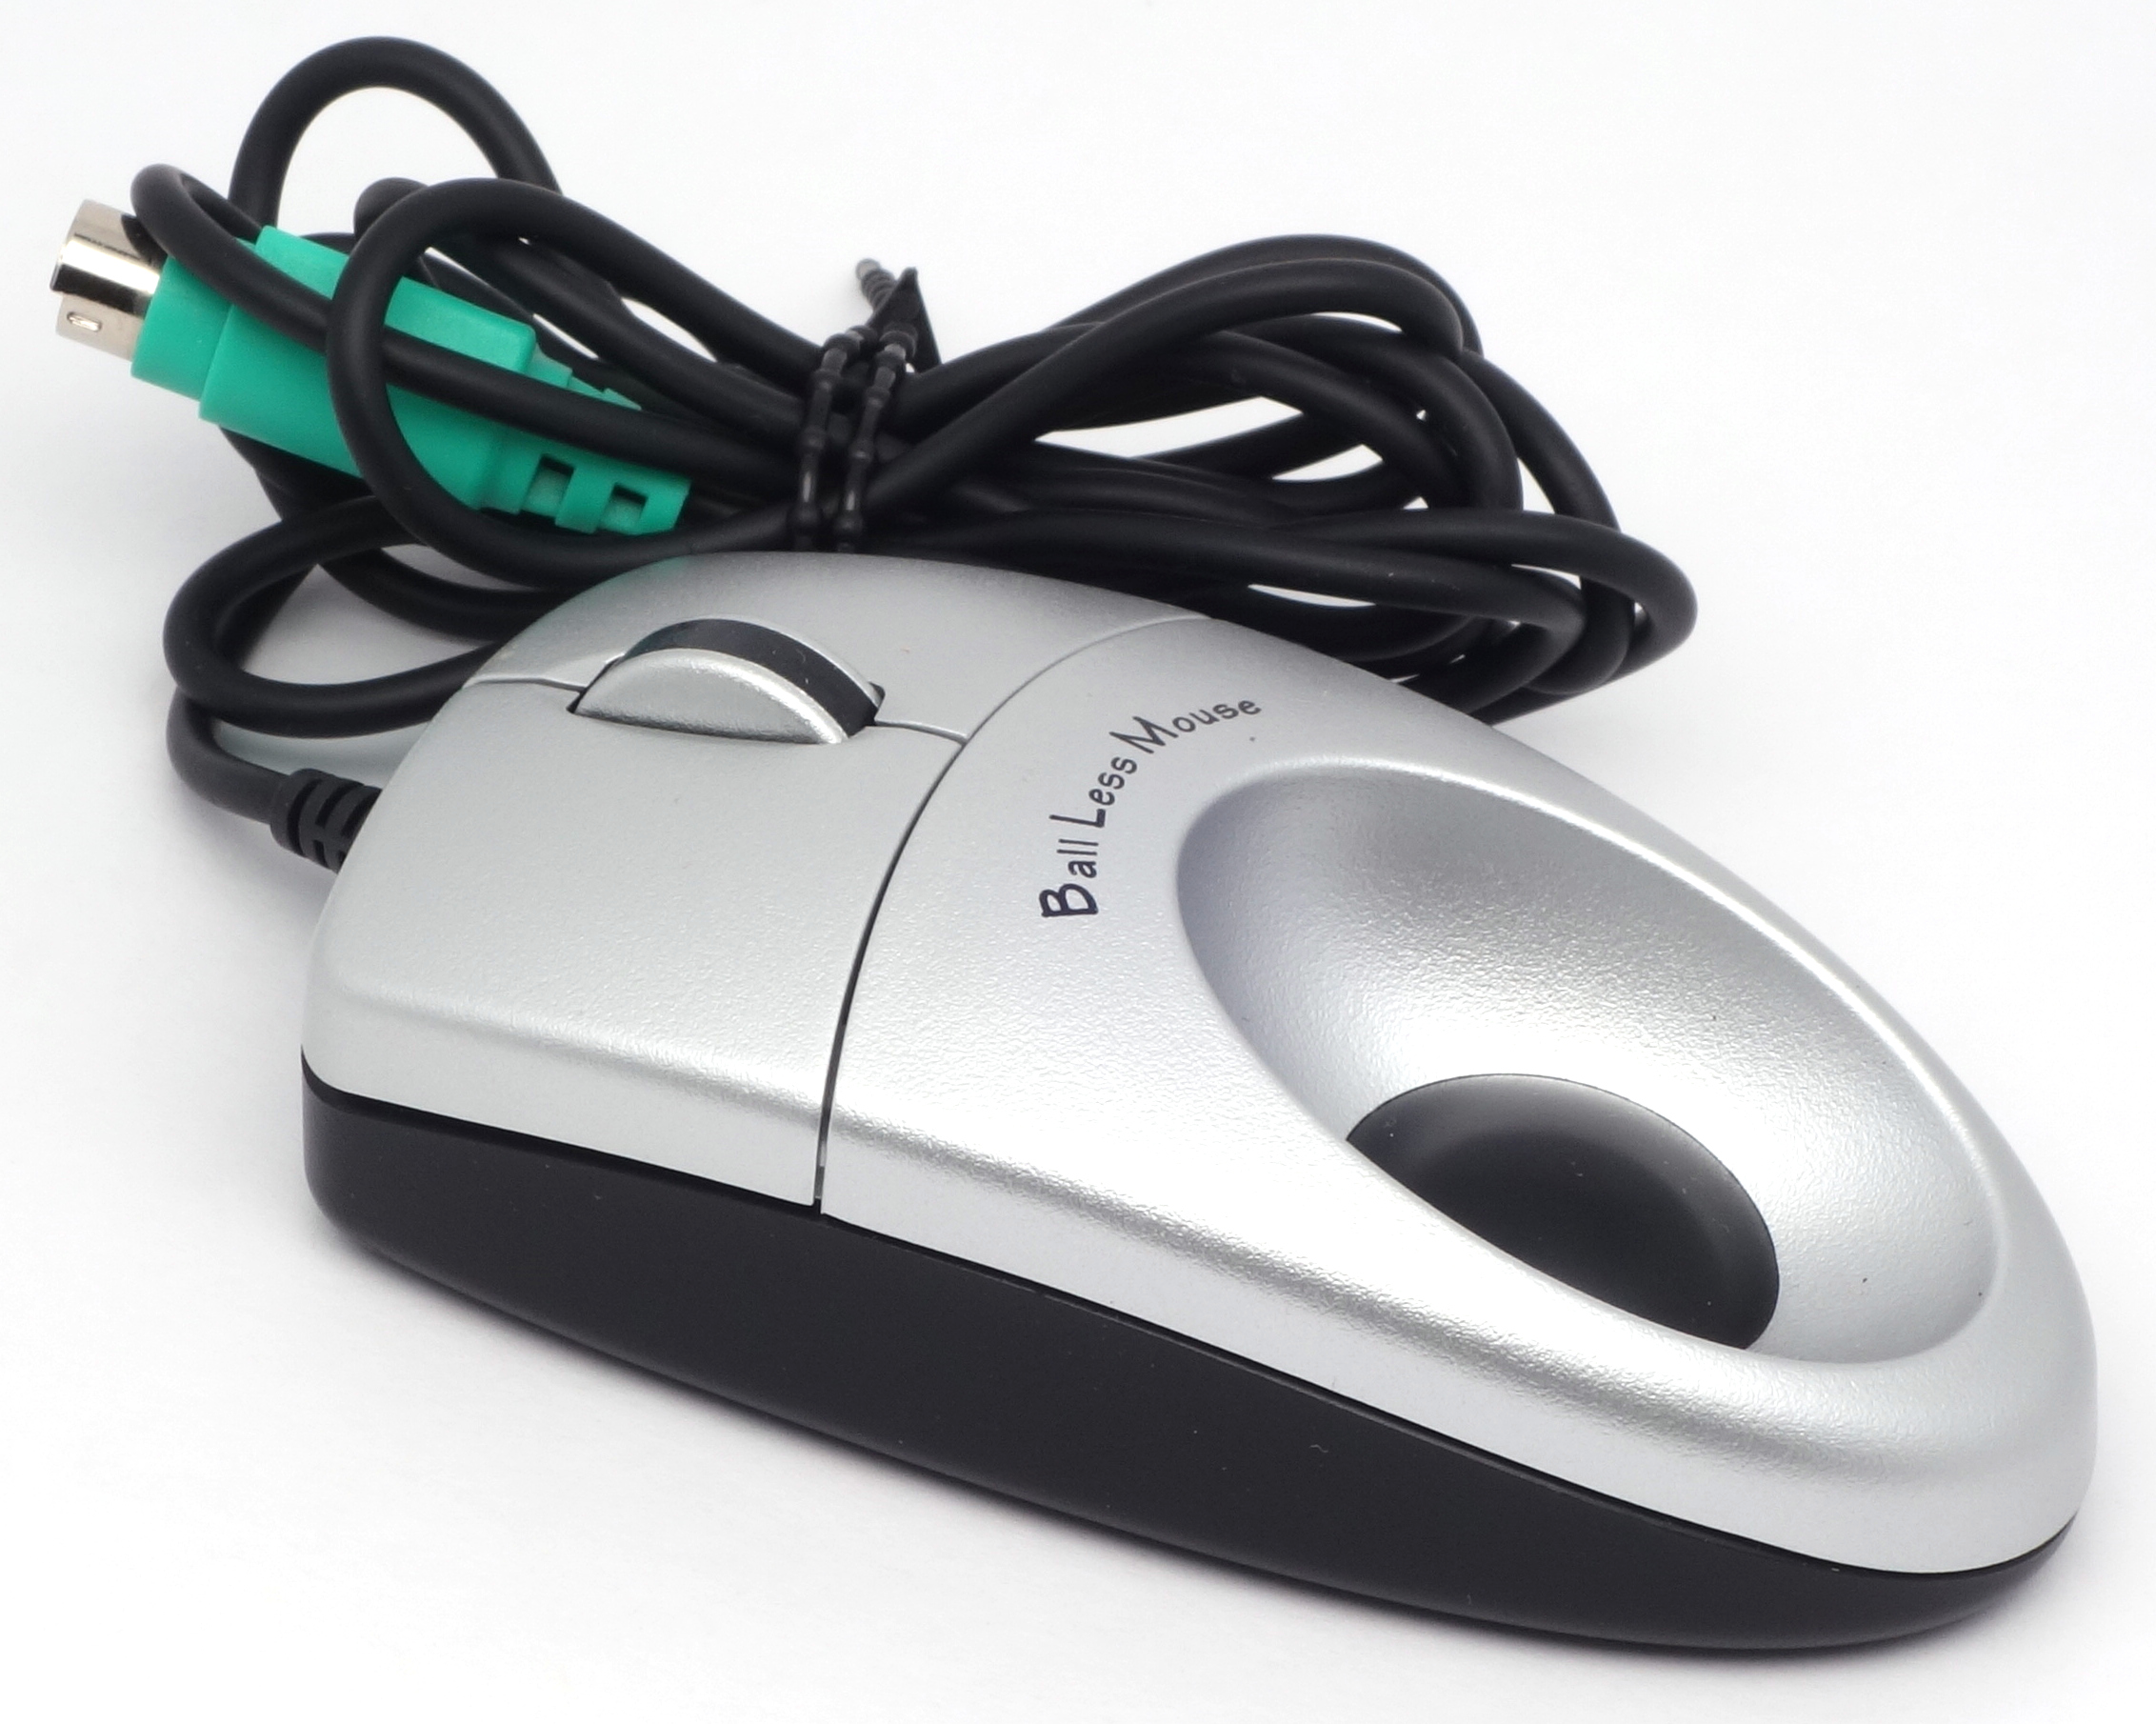
\includegraphics[scale=0.6]{2000_loas_ball_less_mouse/pic_30.jpg}
    \caption{Ball Less Mouse}
    \label{fig:BallLessMousePic}
\end{figure}

According to the Loas website, the mouse was available in three versions: MUS-P241BK (black), MUS-P241SL (silver), and MUS-P241VA (violet and grey) \cite{details}. The manufacturer highlighted the ``direct-drive mechanism'' and ``smooth, stepless scrolling'' as device's unique technical features. The mouse's packaging emphasizes also using two rollers instead of a ball and the consequent lack of any need for cleaning and/or mouse pad \cite{package}.

\section*{Exterior}

The body of the MUS-P241SL mouse features a silver-and-black color scheme and a wedge-shaped silhouette typical of mice from the 2000s: it widens at the button area to maximize their size and narrows smoothly toward the wrist area. The topcase is silver; its half closest to the user contains a decorative area that creatively plays on the absence of a ball. It may visually resemble a cut-open avocado on the top view, but in reality, it is an elongated, spheroidal cavity with a black convex spherical segment at the bottom, symbolizing the missing ball (fig. \ref{fig:BallLessMouseTopBottom}). A curved and grammatically questionable ``Ball Less Mouse'' text can be seen in the center, between this decorative cavity and the buttons. The top view also allows to see a ribbed sleeve protecting the cable, two buttons completely integrated into the shape of the mouse, and a large scroll wheel between them. The scroll wheel is spring-loaded and depresses slightly when pressed, but unlike other mice, it does not function as a third button.

\begin{figure}[h]
    \centering
    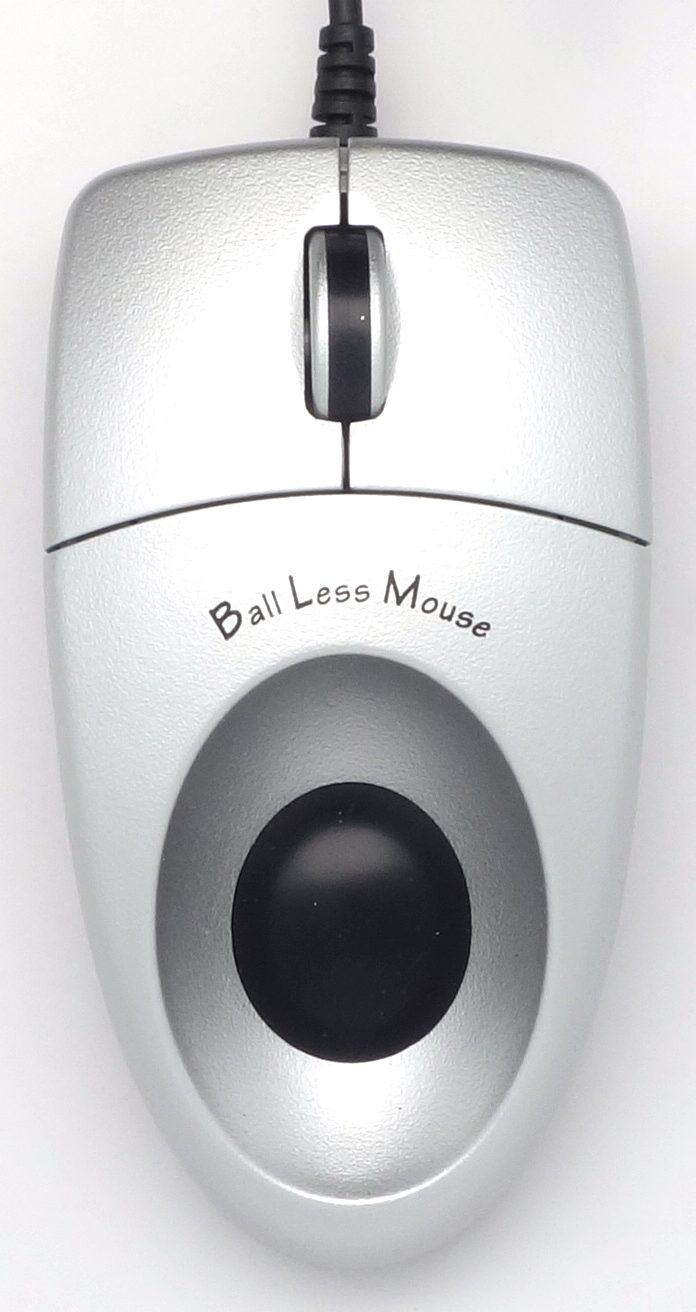
\includegraphics[scale=0.6]{2000_loas_ball_less_mouse/top_30.jpg}
    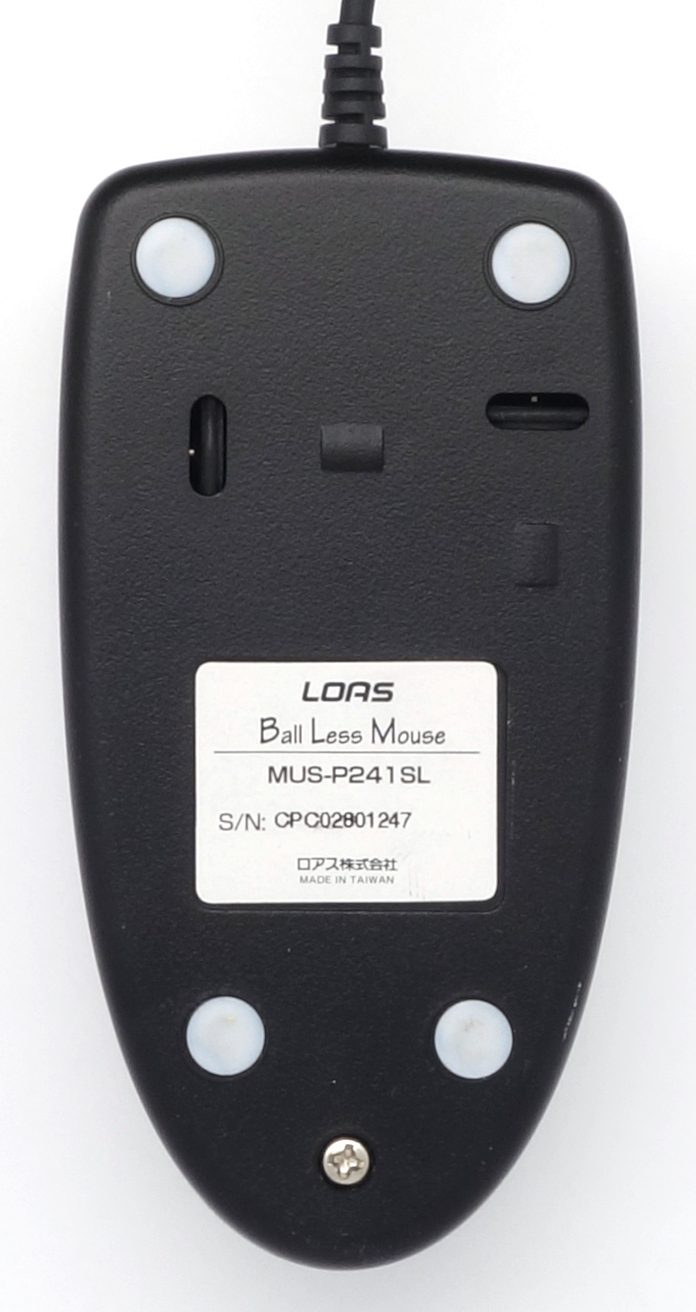
\includegraphics[scale=0.6]{2000_loas_ball_less_mouse/bottom_15.jpg}
    \caption{Ball Less Mouse, top and bottom views}
    \label{fig:BallLessMouseTopBottom}
\end{figure}

The underside of the body is black. It contains a sticker with informational data, round low-friction pads that make the mouse glide easier, as well as two slots through which the motion-tracking wheels protrude. The wheels are positioned orthogonally to one another, so that one always rotates while the other always slides during the longitudinal and lateral movements; additionally, their axes are angled relative to the horizontal plane to better track diagonal movements.

\section*{Size and ergonomics}

Aside from mentioned specifics, Ball Less Mouse is a device of typical size and shape for 2000s (fig. \ref{fig:BallLessMouseSize}). Also, the mouse has a symmetrical shape, equally comfortable for left- and right-handed use.

\begin{figure}[h]
    \centering
    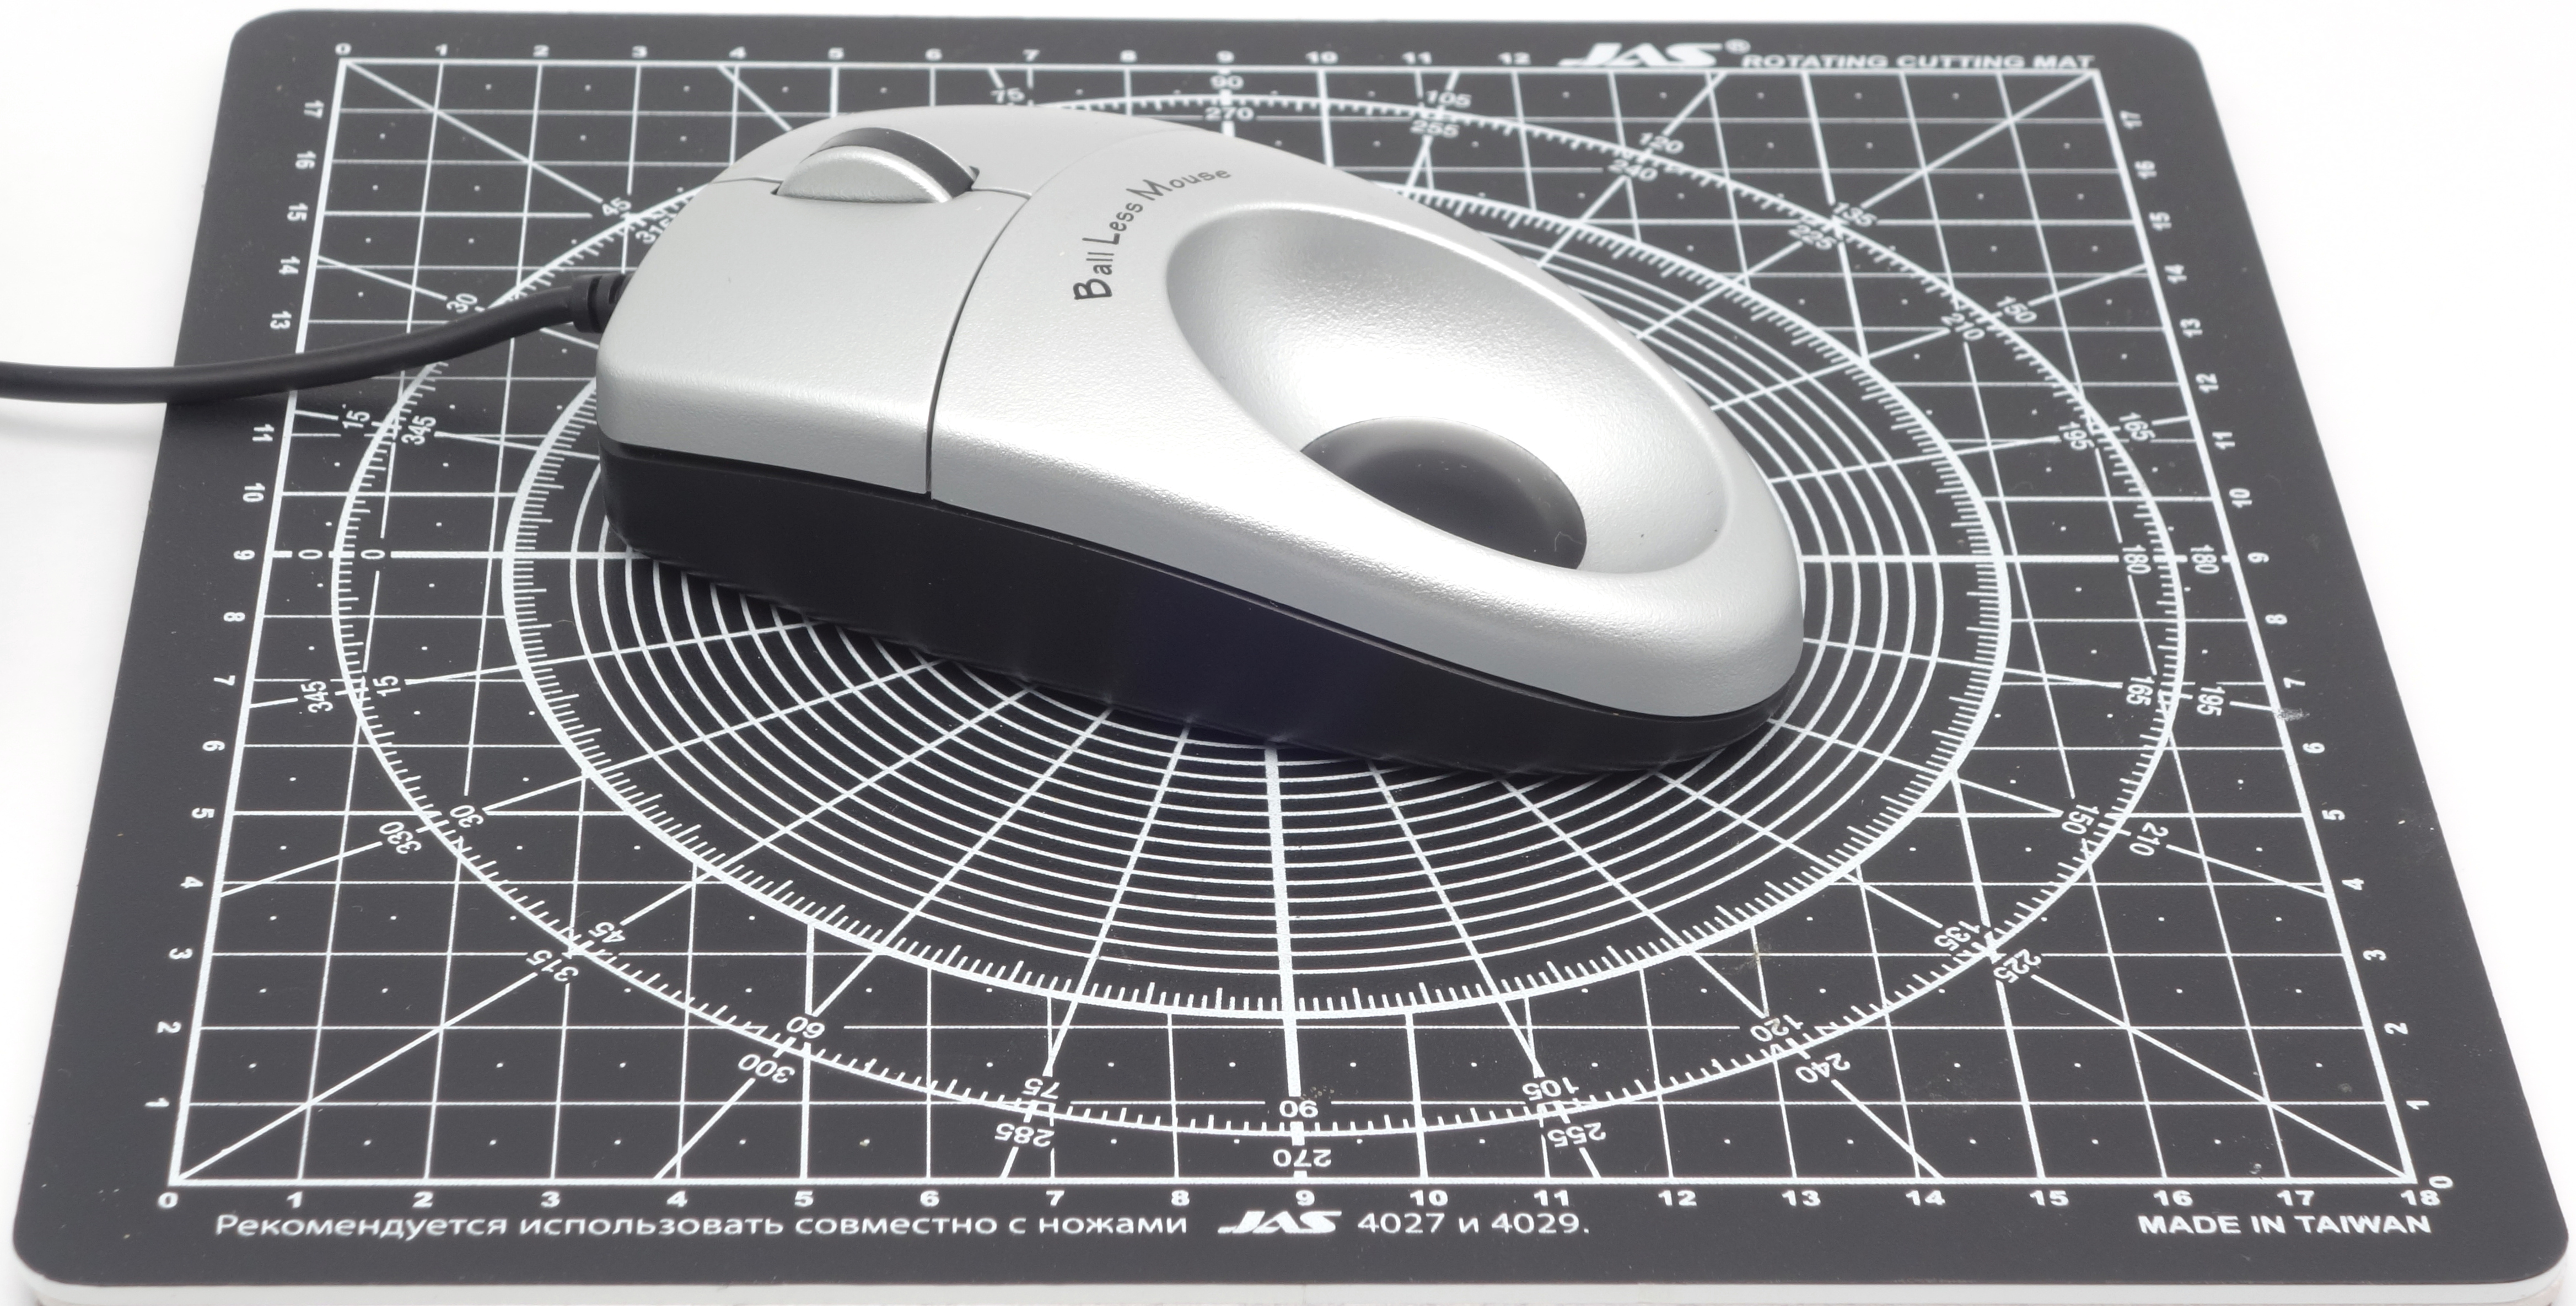
\includegraphics[scale=0.4]{2000_loas_ball_less_mouse/size_15.jpg}
    \caption{Ball Less Mouse on a graduated pad with a grid step of 1~cm}
    \label{fig:BallLessMouseSize}
\end{figure}

The shape of the body and buttons aligned with standards from the 2000s, ensures a comfortable palm position (fig. \ref{fig:BallLessMouseHand}). A ``ball imitation'' cavity built into the topcase is smaller than the user's palm; it is completely covered by the hand and does not significantly affect the usability. 

However, the same cannot be said about the scroll wheel. The user manual carefully specifies that the user can ``scroll the screen up and down by pressing and rotating the wheel'', additionally emphasizing that scrolling requires ``pressing and holding the wheel while turning it'' \cite{manual}. This makes scrolling a significantly more hard process, as it requires additional muscular effort (similar to holding down a button at drag and drop). Clearly, such scrolling mechanism is likely to cause fatigue and pain in the engaged muscles during prolonged, active use.

The user manual also mentions that panoramic scroll by dragging the mouse with pressed third button is not supported, but that's obvious consequence of the mouse having only two buttons.

\begin{figure}[h]
    \centering
    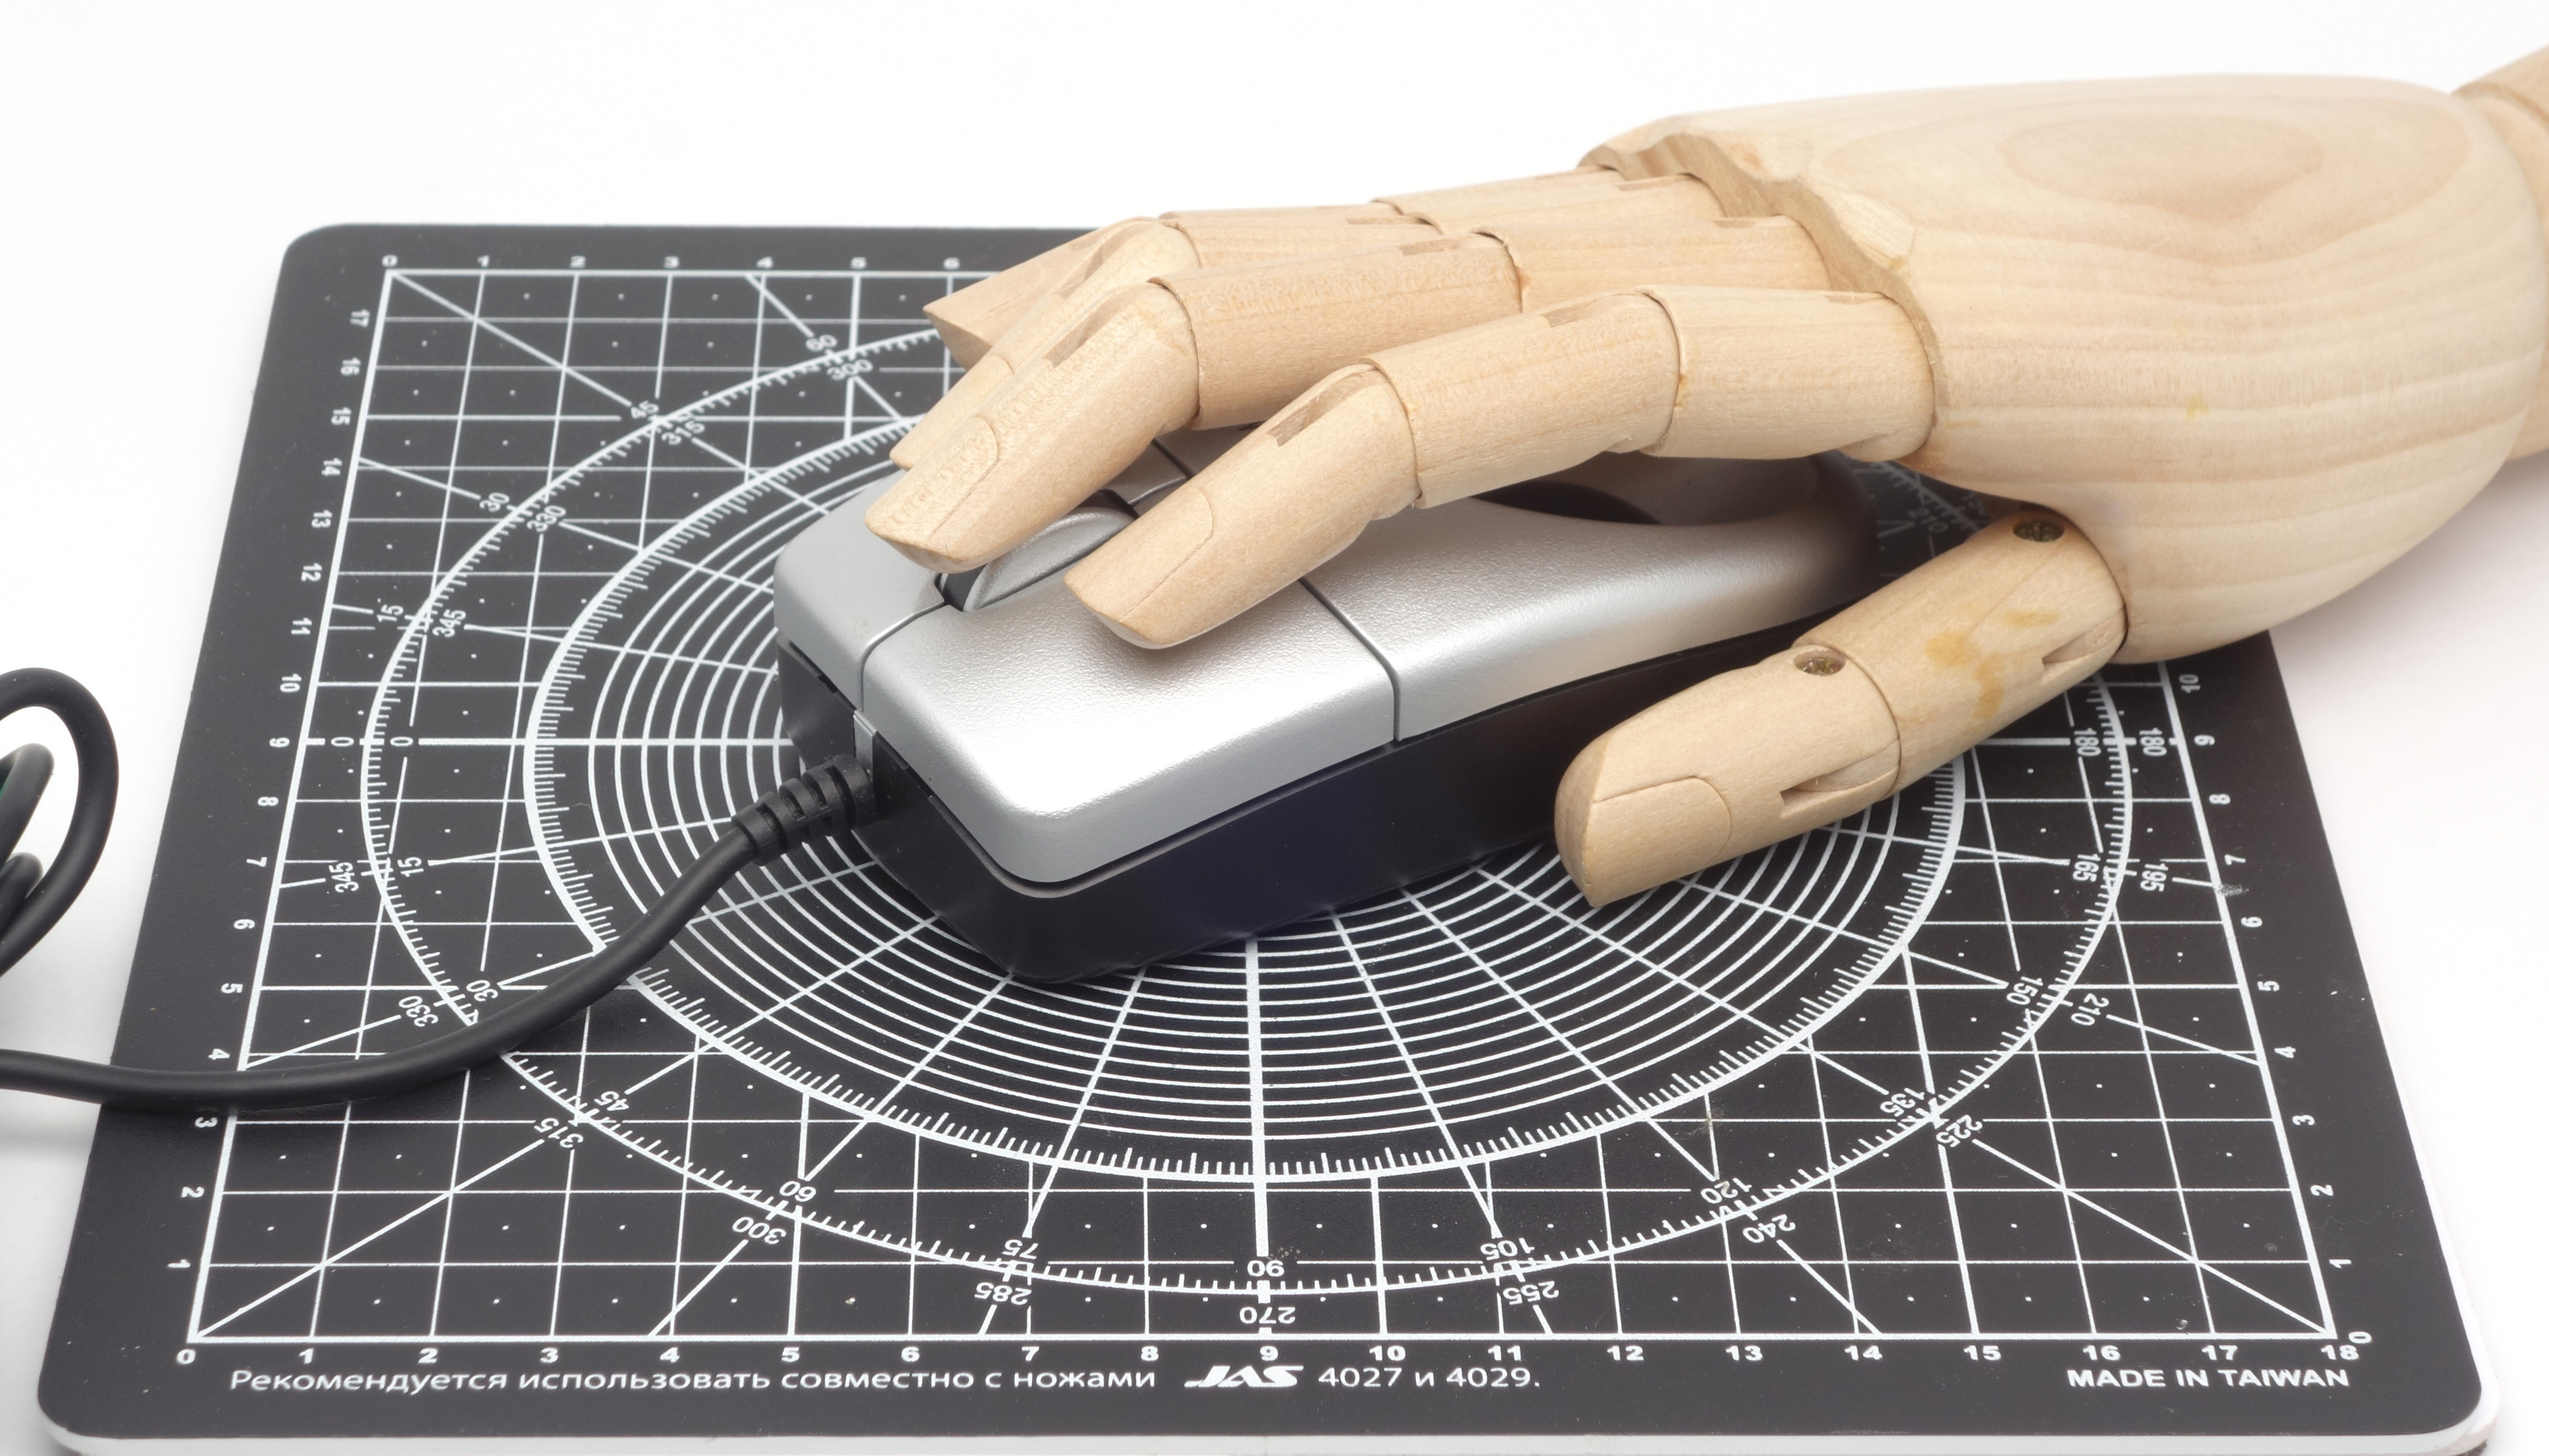
\includegraphics[scale=0.4]{2000_loas_ball_less_mouse/hand_15.jpg}
    \caption{Ball Less Mouse with a human hand model}
    \label{fig:BallLessMouseHand}
\end{figure}

\section*{Connectivity}

According to the description on the company's website \cite{details}, the MUS-P241 mouse was produced exclusively with a PS/2 interface and was intended for use with x86-based computers, such as DOS/V-compatibles and Windows-compatible NEC PC98-NX systems. The manufacturer did not bundle the mouse with any drivers or other software, relying entirely on the operating system's built-in drivers. The list of compatible operating systems included Windows 98, and Windows 2000, as well as Windows 95 with limited functionality (its limitations didn't allow to use scroll wheel).

\section*{Internal design}

The internals of the mouse shown in figure \ref{fig:BallLessMouseInside} allows the mouse to be classified as optomechanical. The design of the optical interrupters is highly unusual: they are cylindrical, with their outer surfaces covered in alternating longitudinal stripes of black and white plastic (unlike traditional optical interrupters, where the working surface is the face of a disk). A dual white housing in the center of the PCB covers two photodetectors and light guides positioned orthogonally to one another. Two LEDs are located outside this housing: the light from each of them reflects off the white stripes on the optical interrupters and travels through the light guides to the photodetectors. Clearly, the use of simple white plastic as a reflective surface was made possible by the increased sensitivity of photodetectors compared to the 1980s, the era of the classic wheeled mouse design.

Mechanically, the mouse replicates the design of the wheeled mice produced in the 1980s: optical encoders are mounted directly onto the wheel axes. This is the design of the Torrignton company, implemented in it's mechanical Manager Mouse and it's variations: TPX Mouse from Tropic Inform\'atica and optical Manager Mouse from Numonics. And, obviously, that is the ``direct-drive mechanism'' mentioned in the mouse's description \cite{details}.

As for the second key feature -- ``smooth operation stepless scrolling'' -- it is caused by the fact that mouse features only two encoders, and one of them serves a dual purpose: scrolling and vertical cursor movement. A spring-loaded encoder mount is used to mechanically separate the scroll wheel from the wheel responsible for cursor vertical movement. When the scroll wheel is pressed, it goes down a bit and contacts the encoder; simultaneously, a spring lifts the axis of the vertical-movement wheel, allowing it to rotate freely without touching the desk surface. The absence of dedicated buttons to disable vertical coordinate transmission during scrolling is likely because the springs themselves perform this function, closing an electrical contact when the scroll wheel is pressed.

Of course, this design does not allow the user to move the cursor vertically while scrolling, but this is an atypical and rarely needed task. In return, it ensures exceptionally smooth scrolling and potentially brings a very precise hi-DPI croll (the feature which is also not necessary in typical user tasks). However, the need to press down on the scroll wheel to scroll remains a significant design drawback.

The mouse resolution is substantially higher than that of its 1980s wheeled predecessors, which is the result of both the  modern microcontroller and the opto-mechanical design, which also features larger wheels; according to the packaging, the resolution of the mouse is 625 DPI \cite{package}.

\begin{figure}[h]
    \centering
    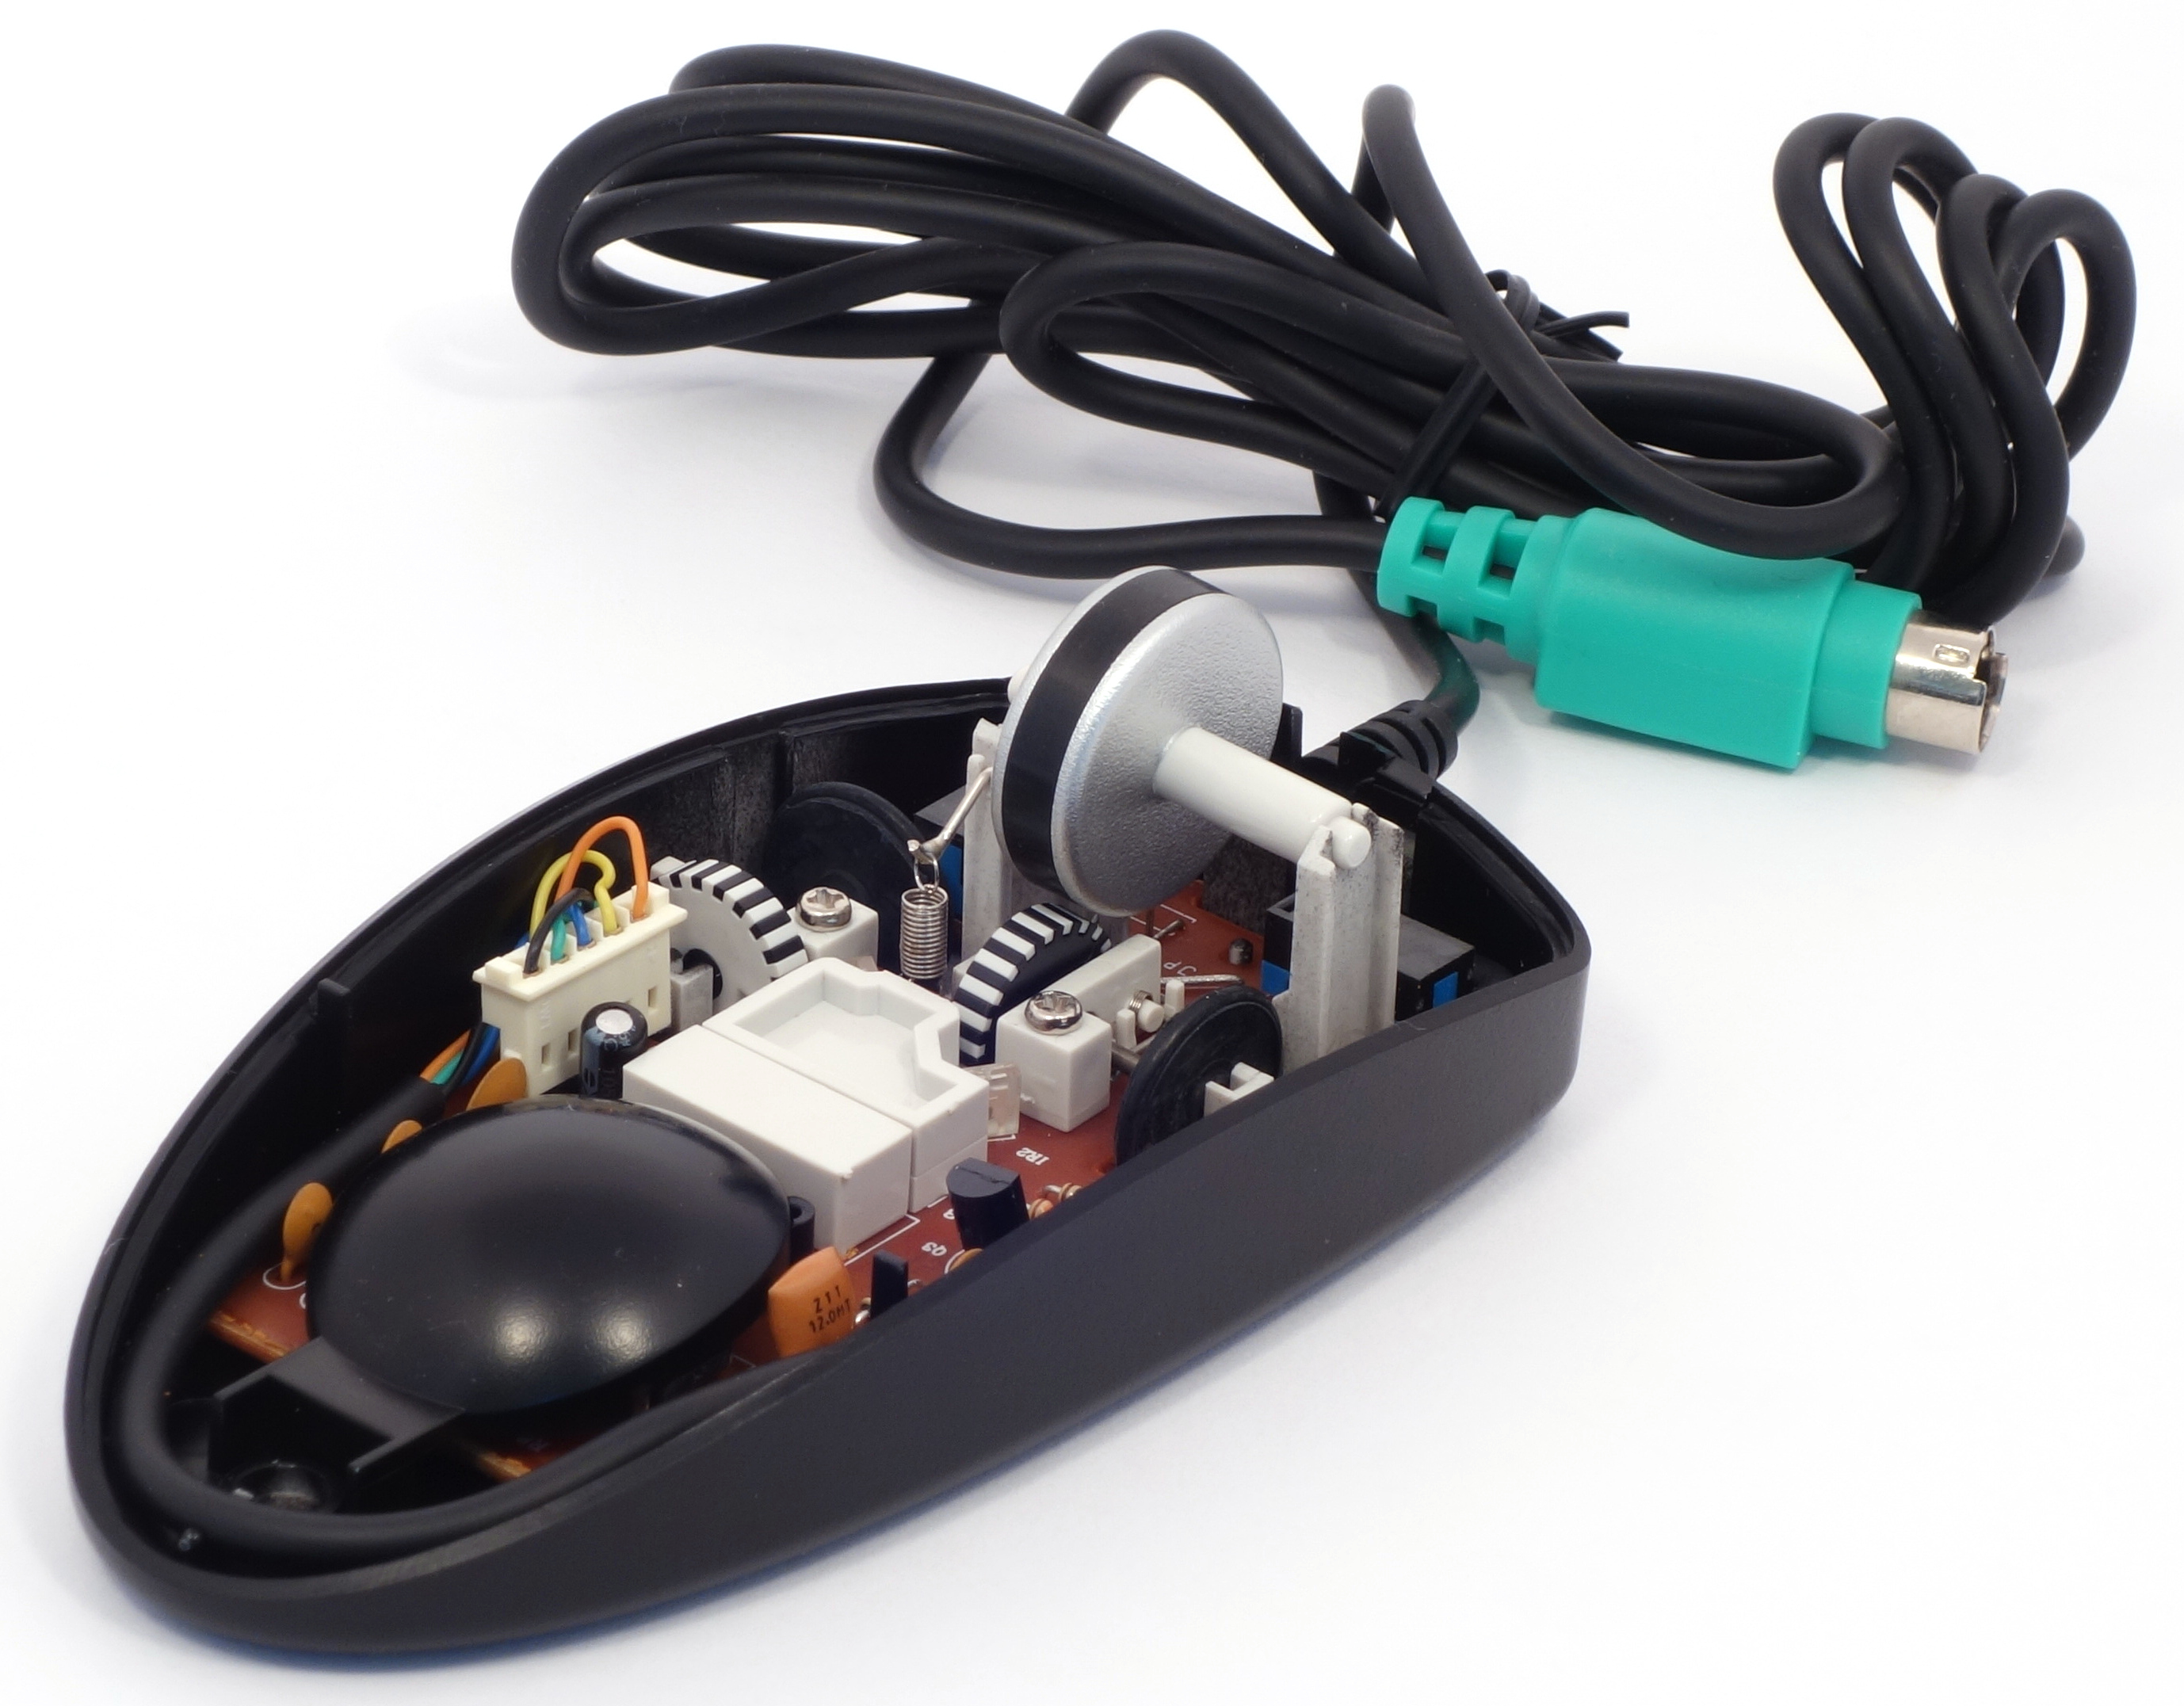
\includegraphics[scale=0.8]{2000_loas_ball_less_mouse/inside_30.jpg}
    \caption{Ball Less Mouse disassembled}
    \label{fig:BallLessMouseInside}
\end{figure}

The markings on the printed circuit board include the strings ``CELLTRIX MOUSE V200031'' and ``Feb 19 Y2K''; this identifies the mouse's manufacturer and (along with the mention of the mouse on the Loas company website \cite{catalog}) dates it to the year 2000.

\begin{thebibliography}{9}
\bibitem{loas} Company profile -- loas.co.jp [in Japanese] \url{https://web.archive.org/web/20010413213735fw_/http://www.loas.co.jp/KA.html}
\bibitem{pat} Transducer for a display-oriented pointing device \url{https://patents.google.com/patent/US3892963A/en}
\bibitem{details} Ballless mouse -- loas.co.jp [in Japanese] \url{https://web.archive.org/web/20010426185102/http://www.loas.co.jp/MUCA7.htm}
\bibitem{package} Ballless mouse cardbox [in Japanese] \url{https://raw.githubusercontent.com/fiowro/mouses/main/source/OCR/loas_mouse_box.pdf}
\bibitem{manual} Ballless mouse cardbox [in Japanese] \url{https://raw.githubusercontent.com/fiowro/mouses/main/source/OCR/loas_mouse_manual.pdf}
\bibitem{catalog} Mouse Catalog -- loas.co.jp [in Japanese] \url{https://web.archive.org/web/20001027054116fw_/http://www.loas.co.jp/MUCA.htm}
\end{thebibliography}
\end{document}
